\title{Boilerplate latex document}
\author{
        Benjamin Bennetzen \\
        Computer Science, 4th semester\\
}
\date{\today}

\documentclass[12pt]{article}

\usepackage{tikz}
\usepackage{mathpartir}
\usepackage{ebproof}
\usepackage{amsmath}
\usepackage{listings}
\usepackage{qtree}
\usepackage{synttree}

\begin{document}
\maketitle

\section{}
\subsection{}
\begin{center}
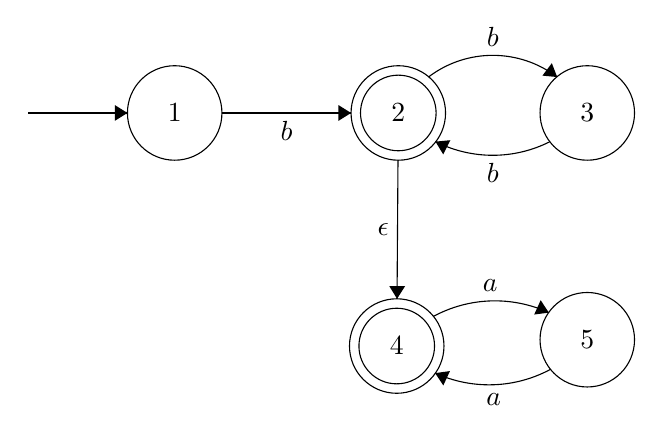
\begin{tikzpicture}[scale=0.2]
\tikzstyle{every node}+=[inner sep=0pt]
\draw [black] (29.9,-15) circle (3);
\draw (29.9,-15) node {$1$};
\draw [black] (44.1,-15) circle (3);
\draw (44.1,-15) node {$2$};
\draw [black] (44.1,-15) circle (2.4);
\draw [black] (56.1,-15) circle (3);
\draw (56.1,-15) node {$3$};
\draw [black] (44,-29.8) circle (3);
\draw (44,-29.8) node {$4$};
\draw [black] (44,-29.8) circle (2.4);
\draw [black] (56.1,-29.4) circle (3);
\draw (56.1,-29.4) node {$5$};
\draw [black] (20.6,-15) -- (26.9,-15);
\fill [black] (26.9,-15) -- (26.1,-14.5) -- (26.1,-15.5);
\draw [black] (32.9,-15) -- (41.1,-15);
\fill [black] (41.1,-15) -- (40.3,-14.5) -- (40.3,-15.5);
\draw (37,-15.5) node [below] {$b$};
\draw [black] (46.012,-12.72) arc (127.29011:52.70989:6.748);
\fill [black] (54.19,-12.72) -- (53.85,-11.84) -- (53.25,-12.63);
\draw (50.1,-10.84) node [above] {$b$};
\draw [black] (53.736,-16.819) arc (-63.11671:-116.88329:8.041);
\fill [black] (46.46,-16.82) -- (46.95,-17.63) -- (47.4,-16.73);
\draw (50.1,-18.19) node [below] {$b$};
\draw [black] (44.08,-18) -- (44.02,-26.8);
\fill [black] (44.02,-26.8) -- (44.53,-26) -- (43.53,-26);
\draw (43.54,-22.4) node [left] {$\epsilon$};
\draw [black] (46.32,-27.924) arc (118.49117:65.2956:8.204);
\fill [black] (53.66,-27.68) -- (53.14,-26.89) -- (52.73,-27.8);
\draw (49.94,-26.4) node [above] {$a$};
\draw [black] (53.778,-31.273) arc (-61.56859:-114.64464:8.216);
\fill [black] (46.44,-31.52) -- (46.96,-32.3) -- (47.38,-31.39);
\draw (50.16,-32.79) node [below] {$a$};
\end{tikzpicture}
\end{center}


\subsection{}
$L_1 \cap L_2 = \{ w \mid \text{w has one b an even number of a's and does not contain the substring ab} \}$

\begin{center}
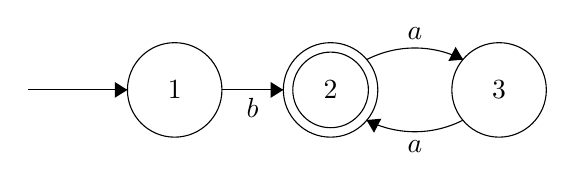
\begin{tikzpicture}[scale=0.2]
\tikzstyle{every node}+=[inner sep=0pt]
\draw [black] (29.9,-15) circle (3);
\draw (29.9,-15) node {$1$};
\draw [black] (39.8,-15) circle (3);
\draw (39.8,-15) node {$2$};
\draw [black] (39.8,-15) circle (2.4);
\draw [black] (50.5,-15) circle (3);
\draw (50.5,-15) node {$3$};
\draw [black] (20.6,-15) -- (26.9,-15);
\fill [black] (26.9,-15) -- (26.1,-14.5) -- (26.1,-15.5);
\draw [black] (42.076,-13.084) arc (117.27854:62.72146:6.707);
\fill [black] (48.22,-13.08) -- (47.74,-12.27) -- (47.28,-13.16);
\draw (45.15,-11.84) node [above] {$a$};
\draw [black] (48.221,-16.913) arc (-62.78812:-117.21188:6.716);
\fill [black] (42.08,-16.91) -- (42.56,-17.72) -- (43.02,-16.83);
\draw (45.15,-18.16) node [below] {$a$};
\draw [black] (32.9,-15) -- (36.8,-15);
\fill [black] (36.8,-15) -- (36,-14.5) -- (36,-15.5);
\draw (34.85,-15.5) node [below] {$b$};
\end{tikzpicture}
\end{center}


\subsection{}
We will start be converting the NFA to a GNFA.

\begin{center}
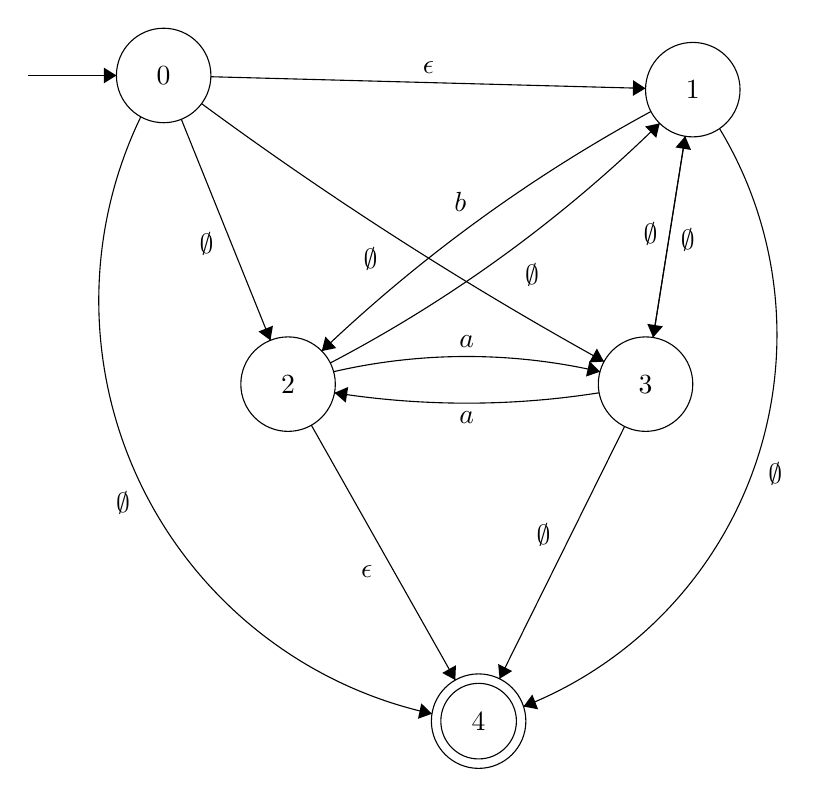
\begin{tikzpicture}[scale=0.2]
\tikzstyle{every node}+=[inner sep=0pt]
\draw [black] (52.2,-8.8) circle (3);
\draw (52.2,-8.8) node {$1$};
\draw [black] (26.5,-27.5) circle (3);
\draw (26.5,-27.5) node {$2$};
\draw [black] (49.2,-27.5) circle (3);
\draw (49.2,-27.5) node {$3$};
\draw [black] (38.6,-48.9) circle (3);
\draw (38.6,-48.9) node {$4$};
\draw [black] (38.6,-48.9) circle (2.4);
\draw [black] (18.6,-7.9) circle (3);
\draw (18.6,-7.9) node {$0$};
\draw [black] (29.393,-26.709) arc (103.01282:76.98718:37.559);
\fill [black] (46.31,-26.71) -- (45.64,-26.04) -- (45.42,-27.02);
\draw (37.85,-25.24) node [above] {$a$};
\draw [black] (46.251,-28.05) arc (-81.03641:-98.96359:53.92);
\fill [black] (29.45,-28.05) -- (30.16,-28.67) -- (30.32,-27.68);
\draw (37.85,-29.21) node [below] {$a$};
\draw [black] (28.639,-25.397) arc (133.63599:118.44527:97.783);
\fill [black] (28.64,-25.4) -- (29.56,-25.21) -- (28.87,-24.48);
\draw (37.44,-16.6) node [above] {$b$};
\draw [black] (10,-7.9) -- (15.6,-7.9);
\fill [black] (15.6,-7.9) -- (14.8,-7.4) -- (14.8,-8.4);
\draw [black] (21.6,-7.98) -- (49.2,-8.72);
\fill [black] (49.2,-8.72) -- (48.41,-8.2) -- (48.39,-9.2);
\draw (35.42,-7.82) node [above] {$\epsilon$};
\draw [black] (27.98,-30.11) -- (37.12,-46.29);
\fill [black] (37.12,-46.29) -- (37.16,-45.35) -- (36.29,-45.84);
\draw (31.89,-39.42) node [left] {$\epsilon$};
\draw [black] (19.72,-10.68) -- (25.38,-24.72);
\fill [black] (25.38,-24.72) -- (25.54,-23.79) -- (24.62,-24.16);
\draw (21.8,-18.59) node [left] {$\emptyset$};
\draw [black] (46.565,-26.066) arc (-118.92117:-126.35982:233.966);
\fill [black] (46.56,-26.07) -- (46.11,-25.24) -- (45.62,-26.12);
\draw (31.74,-18.79) node [below] {$\emptyset$};
\draw [black] (35.639,-48.43) arc (-102.22494:-205.76837:26.845);
\fill [black] (35.64,-48.43) -- (34.96,-47.77) -- (34.75,-48.75);
\draw (16.49,-35.05) node [left] {$\emptyset$};
\draw [black] (47.87,-30.19) -- (39.93,-46.21);
\fill [black] (39.93,-46.21) -- (40.73,-45.72) -- (39.84,-45.27);
\draw (43.2,-37.1) node [left] {$\emptyset$};
\draw [black] (49.68,-24.54) -- (51.72,-11.76);
\fill [black] (51.72,-11.76) -- (51.1,-12.47) -- (52.09,-12.63);
\draw (51.41,-18.36) node [right] {$\emptyset$};
\draw [black] (51.72,-11.76) -- (49.68,-24.54);
\fill [black] (49.68,-24.54) -- (50.3,-23.83) -- (49.31,-23.67);
\draw (49.99,-17.94) node [left] {$\emptyset$};
\draw [black] (50.096,-10.938) arc (-45.51446:-62.40429:88.059);
\fill [black] (50.1,-10.94) -- (49.17,-11.14) -- (49.88,-11.86);
\draw (41.99,-19.82) node [below] {$\emptyset$};
\draw [black] (53.898,-11.271) arc (31.1138:-68.58275:25.352);
\fill [black] (41.45,-47.97) -- (42.38,-48.15) -- (42.01,-47.21);
\draw (56.97,-33.23) node [right] {$\emptyset$};
\end{tikzpicture}
\end{center}


\begin{center}
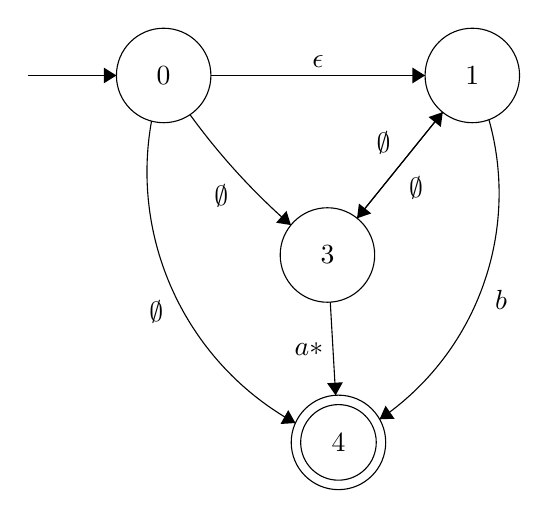
\begin{tikzpicture}[scale=0.2]
\tikzstyle{every node}+=[inner sep=0pt]
\draw [black] (47,-13.8) circle (3);
\draw (47,-13.8) node {$1$};
\draw [black] (37.8,-25.2) circle (3);
\draw (37.8,-25.2) node {$3$};
\draw [black] (38.5,-37.1) circle (3);
\draw (38.5,-37.1) node {$4$};
\draw [black] (38.5,-37.1) circle (2.4);
\draw [black] (27.4,-13.8) circle (3);
\draw (27.4,-13.8) node {$0$};
\draw [black] (18.8,-13.8) -- (24.4,-13.8);
\fill [black] (24.4,-13.8) -- (23.6,-13.3) -- (23.6,-14.3);
\draw [black] (30.4,-13.8) -- (44,-13.8);
\fill [black] (44,-13.8) -- (43.2,-13.3) -- (43.2,-14.3);
\draw (37.2,-13.3) node [above] {$\epsilon$};
\draw [black] (35.475,-23.305) arc (-131.20901:-144.04381:42.486);
\fill [black] (35.48,-23.3) -- (35.2,-22.4) -- (34.54,-23.15);
\draw (31.54,-21.44) node [left] {$\emptyset$};
\draw [black] (35.765,-35.875) arc (-118.85487:-190.19935:18.215);
\fill [black] (35.77,-35.87) -- (35.31,-35.05) -- (34.82,-35.93);
\draw (27.4,-28.82) node [left] {$\emptyset$};
\draw [black] (37.98,-28.19) -- (38.32,-34.11);
\fill [black] (38.32,-34.11) -- (38.78,-33.28) -- (37.78,-33.34);
\draw (37.56,-31.18) node [left] {$a*$};
\draw [black] (39.68,-22.87) -- (45.12,-16.13);
\fill [black] (45.12,-16.13) -- (44.22,-16.44) -- (45,-17.07);
\draw (42.96,-20.93) node [right] {$\emptyset$};
\draw [black] (45.12,-16.13) -- (39.68,-22.87);
\fill [black] (39.68,-22.87) -- (40.58,-22.56) -- (39.8,-21.93);
\draw (41.84,-18.07) node [left] {$\emptyset$};
\draw [black] (48.055,-16.604) arc (15.67001:-55.75465:17.351);
\fill [black] (41.11,-35.63) -- (42.06,-35.6) -- (41.49,-34.77);
\draw (48.41,-28.03) node [right] {$b$};
\end{tikzpicture}
\end{center}


\section{}
\begin{lstlisting}
S -> T | S : T
T -> T * F * T | <empty>
F -> a | [S]
\end{lstlisting}

\begin{lstlisting}
S -> S : T
  -> T * F * T : T
  -> T * F * T * F * T : T
  ->

S -> T ->

S -> S : T
  -> S : T : T
  -> T : T : T
  -> : T * F * T :
  -> : * F * T :
  -> : * a * T :
  -> : * a * :
\end{lstlisting}

\synttree
[S
  [S
    [S
      [T
        [empty]
      ]
    ]
    [\text{:}]
    [T]
  ]
  [\text{:}]
  [T]
]


\begin{mathpar}
\inferrule[Foo]{A \\ B \\\\ C}{D}
\and
\inferrule[Bar]{X}{Y}
\end{mathpar}

\begin{prooftree}
%1st branch
        \infer0[by (Env \(\nothing\))]{\nothing \vdash \diamond}
        \infer1[by (Type Const)]{\nothing \vdash K}
        \infer0[by (Env \(\nothing\))]{\nothing \vdash \diamond}
        \infer1[by (Type Const)]{\nothing \vdash K}
        \infer2[by (Type Arrow)]{\nothing \vdash K \to K}
        \infer1[by (Env \(x\))]{\nothing, y: K \to K  \vdash  \diamond}
        \infer1[by (Type Const)]{\nothing, y: K \to K  \vdash  K}
        \infer1[by (Env \(x\))]{\nothing, y: K \to K, z:K  \vdash \diamond}
        \infer1[by (Val \(x\))]{\nothing, y: K \to K, z:K  \vdash y : K \to K}
        % 2nd branch
        \infer0[by (Env \(\nothing\))]{\nothing \vdash \diamond}
        \infer1[by (Type Const)]{\nothing \vdash K}
        \infer0[by (Env \(\nothing\))]{\nothing \vdash \diamond}
        \infer1[by (Type Const)]{\nothing \vdash K}
        \infer2[by (Type Arrow)]{\nothing \vdash K \to K}
        \infer1[by (Env \(x\))]{\nothing, y: K \to K  \vdash  \diamond}
        \infer1[by (Type Const)]{\nothing, y: K \to K  \vdash  K}
        \infer1[by (Env \(x\))]{\nothing, y: K \to K, z:K  \vdash \diamond}
        \infer1[by (Val \(x\))]{\nothing, y: K \to K, z:K  \vdash z : K \to K}
        % Conclusion
        \infer2[by (Val Appl)]{\nothing, y: K \to K, z:K  \vdash y(z) : K}
        \infer1[by (Val Fun)]{\nothing, y: K \to K, z:K  \vdash \lambda z : K.y(z) : K \to K}
\end{prooftree}

\end{document}
